\chapter{Results}
This section goes through how the final implementation results in a software that solves the proposed objectives. Section (ref screenshots) includes screenshots showing the globe browsing in use.

The benchmarks were done using an relatively old consumer laptop computer. Its specs are provided below.

\begin{table}[h]
  \centering
  \caption[]{Computer used for Benchmarking}
    \label{table:benchmark host}
  \begin{tabular}{| r l |}
    \hline
      \textbf{Computer Model:}  & MacBook Pro (15'' early 2011) \\
      \textbf{Processor:}       & 2GHz Intel Core i7 \\
      \textbf{RAM:}             & 8 GB 1333MHz DDR3 RAM \\
      \textbf{Graphics:}        & AMD Radeon HD 6490M 256 MB \\
    \hline
  \end{tabular}
\end{table}

\clearpage
\section{Zooming In}
\FloatBarrier
The chunk rendering algorithm was evaluated for a top down view at different distances to the ground. The settings for the evaluation are presented in Table \ref{table:settingstopdown}, the camera views for the evaluation points are shown in Figure \ref{fig:topdown} and the results are presented in Figure \ref{fig:topdowngraph}.
\begin{table}[h]
  \centering
  \caption[]{Top down settings}
    \label{table:settingstopdown}
  \begin{tabular}{| r l |}
    \hline
      \textbf{Globe:}             & Earth \\
      \textbf{Map datasets:}      & HeightLayers=[GCS\_Elevation\footnote{http://services.arcgisonline.com/ArcGIS/rest/services/ESRI\_Imagery\_World\_2D/MapServer}] \\
                                  & ColorLayers=[ESRI\_World\_2D\footnote{http://198.102.45.23/arcgis/rest/services/worldelevation3d/terrain3d?}] \\
      \textbf{LOD Scale factor:}  & 10.0 \\
      \textbf{LOD Evaluation:}    & By distance \\
      \textbf{Culling:}           & Frustum culling, Horizon culling \\
      \textbf{Level blending:}    & Enabled \\
      \textbf{Camera View:}       & Facing down, varying altitudes\\
    \hline
  \end{tabular}
\end{table}

\begin{figure}[h]
    \centering
    \begin{subfigure}[bt]{0.31\textwidth}
        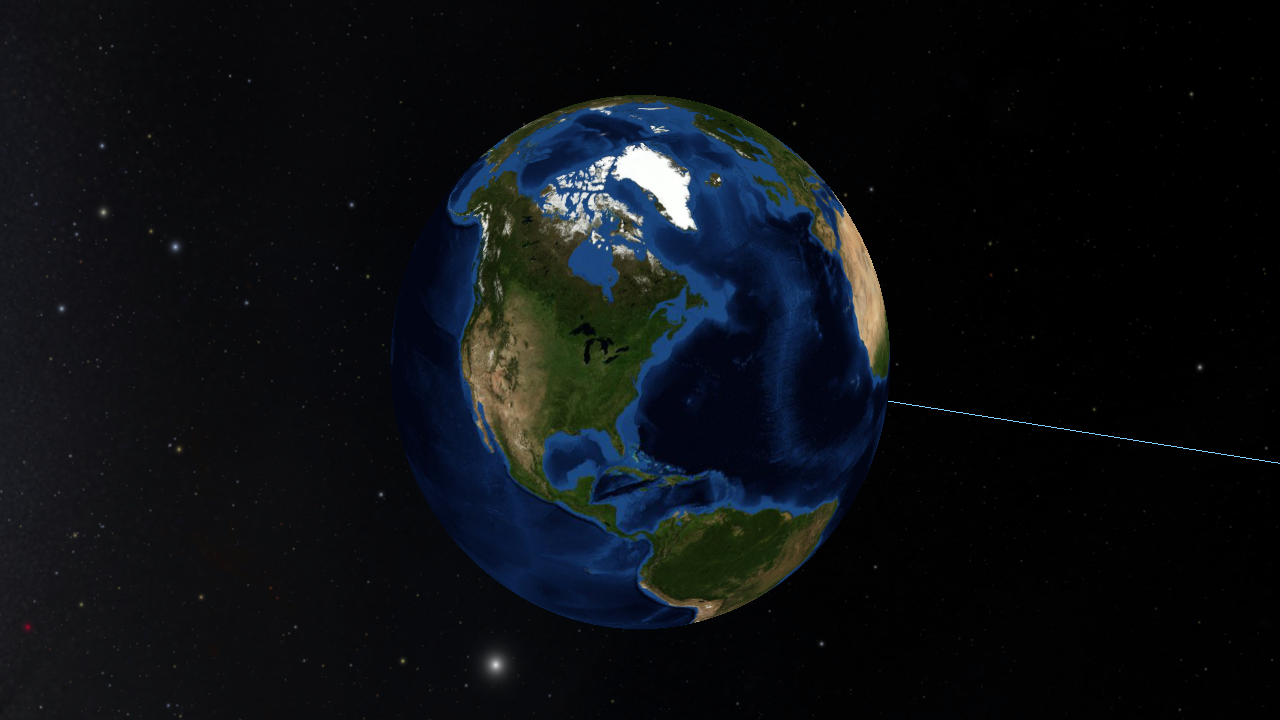
\includegraphics[width=\textwidth]{figures/results/topdown/topdown5.png}
        \caption{Earth}
    \end{subfigure}
    ~
    \begin{subfigure}[bt]{0.31\textwidth}
        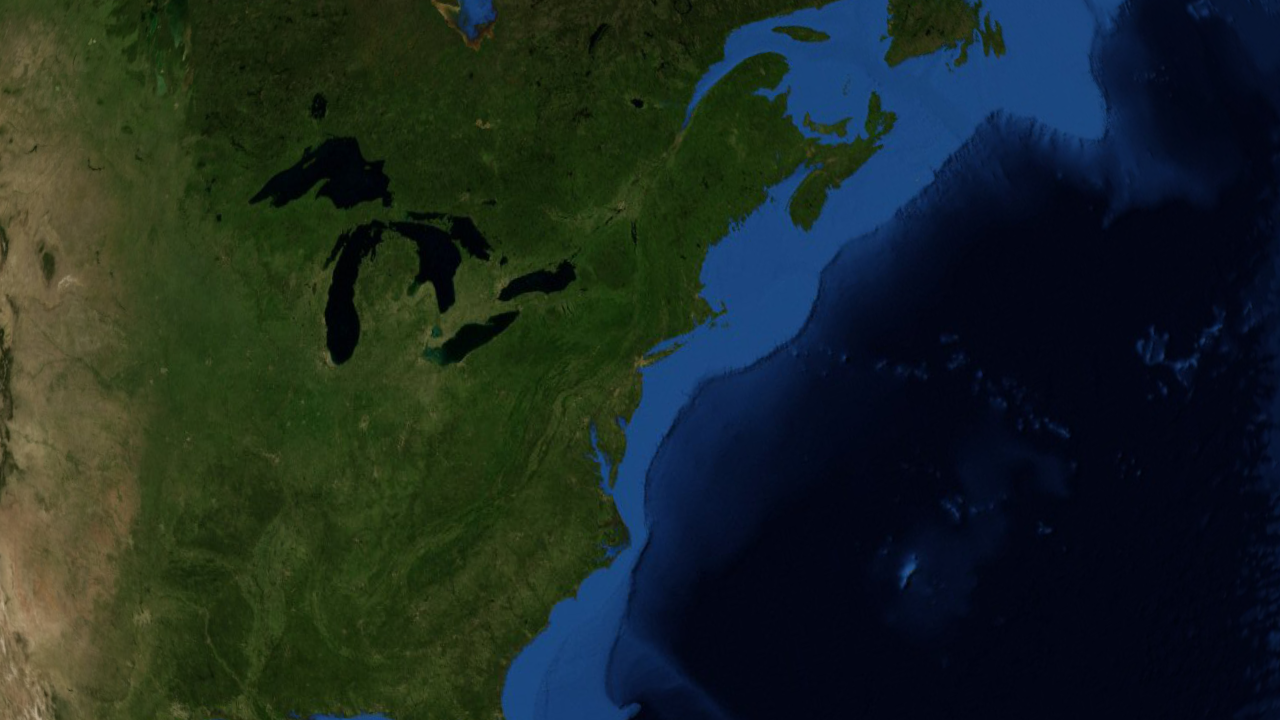
\includegraphics[width=\textwidth]{figures/results/topdown/topdown4.png}
        \caption{East America}
    \end{subfigure}
    ~
    \begin{subfigure}[bt]{0.31\textwidth}
        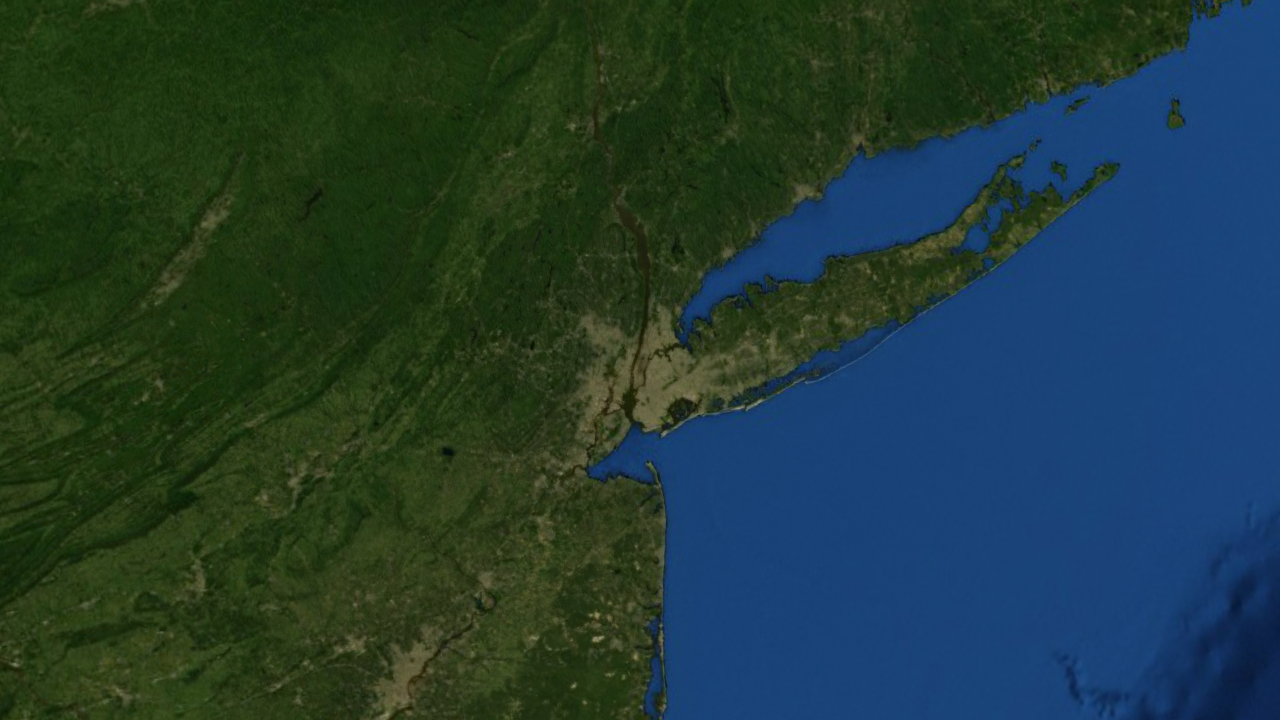
\includegraphics[width=\textwidth]{figures/results/topdown/topdown3.png}
        \caption{New York City}
    \end{subfigure}
    ~
    \begin{subfigure}[bt]{0.31\textwidth}
        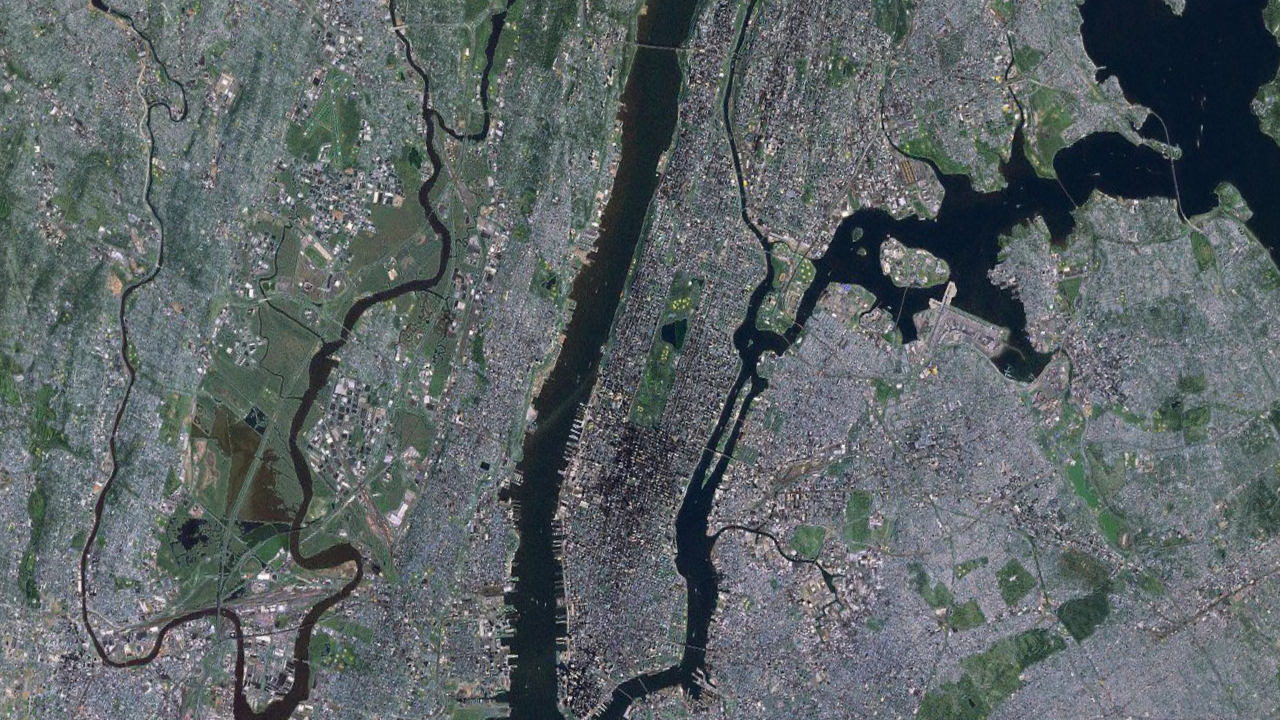
\includegraphics[width=\textwidth]{figures/results/topdown/topdown2.png}
        \caption{Manhattan}
    \end{subfigure}
    ~
    \begin{subfigure}[bt]{0.31\textwidth}
        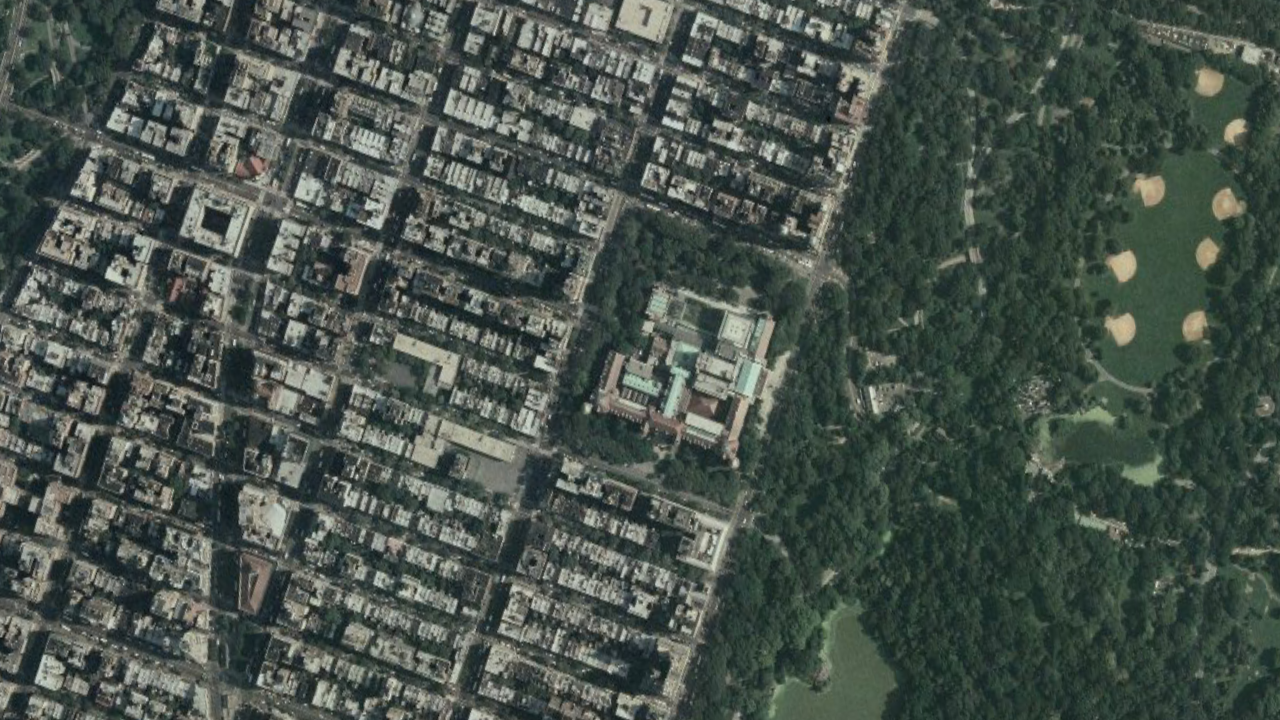
\includegraphics[width=\textwidth]{figures/results/topdown/topdown1.png}
        \caption{Central Park}
    \end{subfigure}
    \caption{Top-down views of Earth at different zoom levels}
    \label{fig:topdown}
\end{figure}

\begin{figure}[h]
\begin{tikzpicture}
    \begin{axis}[
        width  = 1.0*\textwidth,
        height = 12cm,
        major x tick style = transparent,
        ybar=2*\pgflinewidth,
        bar width=8pt,
        ymajorgrids = true,
        %ylabel = {Number of},
        symbolic x coords={Earth, East America, NYC, Manhattan, Central Park},
        xtick = data,
        scaled y ticks = false,
        enlarge x limits=0.25,
        ymin=0,
        legend cell align=left,
        legend style={
                at={(0.43, 0.66)},
                anchor=south east,
                column sep=1ex
        }
    ]

      \addplot[style={chunks_color,fill=chunks_color,mark=none}]
        coordinates { (Earth, 10) (East America, 70) (NYC, 70) (Manhattan, 110) (Central Park, 142) };

      \addplot[style={leafs_color,fill=leafs_color,mark=none}]
        coordinates { (Earth, 8) (East America, 53) (NYC, 53) (Manhattan, 83) (Central Park, 107) };
      
      \addplot[style={rendered_color,fill=rendered_color,mark=none}]
        coordinates { (Earth, 7) (East America, 14) (NYC, 13) (Manhattan, 17) (Central Park, 11) };

      \addplot[style={globe_render_time,fill=globe_render_time,mark=none}]
        coordinates { (Earth, 17) (East America, 20) (NYC, 20) (Manhattan, 21) (Central Park, 21) };

      \addplot[style={frame_render_time,fill=frame_render_time,mark=none}]
        coordinates { (Earth, 1.1) (East America, 3.4) (NYC, 3.5) (Manhattan, 5) (Central Park, 5.6) };

      \legend{Chunks, Leaf chunks, Rendered chunks, Frame time [ms], Globe render time [ms]}

    \end{axis}
\end{tikzpicture}
\caption{}
\label{fig:topdowngraph}
\end{figure}



\clearpage
\section{Culling for distance based LOD}
\FloatBarrier
The culling algorithms Frustum culling and Horizon Culling were compared and evaluated. The settings used are provided in Table \ref{table:cullingd}. Note that LOD evaluation is done by distance. Figure \ref{fig:cullingdcam} shows the camera view evaluated. Figure \ref{fig:cullingd} shows and overview of the rendered chunks using the different culling and benchmarks are listed in Table \ref{table:cullingd}.

\begin{table}[h]
  \centering
  \caption[]{Culling test}
    \label{table:cullingd}
  \begin{tabular}{| r l |}
    \hline
      \textbf{Globe:}             & Earth \\
      \textbf{Map datasets:}      & HeightLayers=[GCS\_Elevation\footnote{http://services.arcgisonline.com/ArcGIS/rest/services/ESRI\_Imagery\_World\_2D/MapServer}] \\
                                  & ColorLayers=[ESRI\_World\_2D\footnote{http://198.102.45.23/arcgis/rest/services/worldelevation3d/terrain3d?}] \\
      \textbf{LOD Scale factor:}  & 7.8 \\
      \textbf{LOD Evaluation:}    & By distance \\
      \textbf{Culling:}           & \textbf{Evaluated} \\
      \textbf{Level blending:}    & Enabled \\
      \textbf{Camera View:}       & Looking towards western horizon\\
      \textbf{Location:}          & New York, New Jersey\\
    \hline
  \end{tabular}
\end{table}

\begin{figure}[h]
    \centering
    \begin{subfigure}[bt]{1.0\textwidth}
        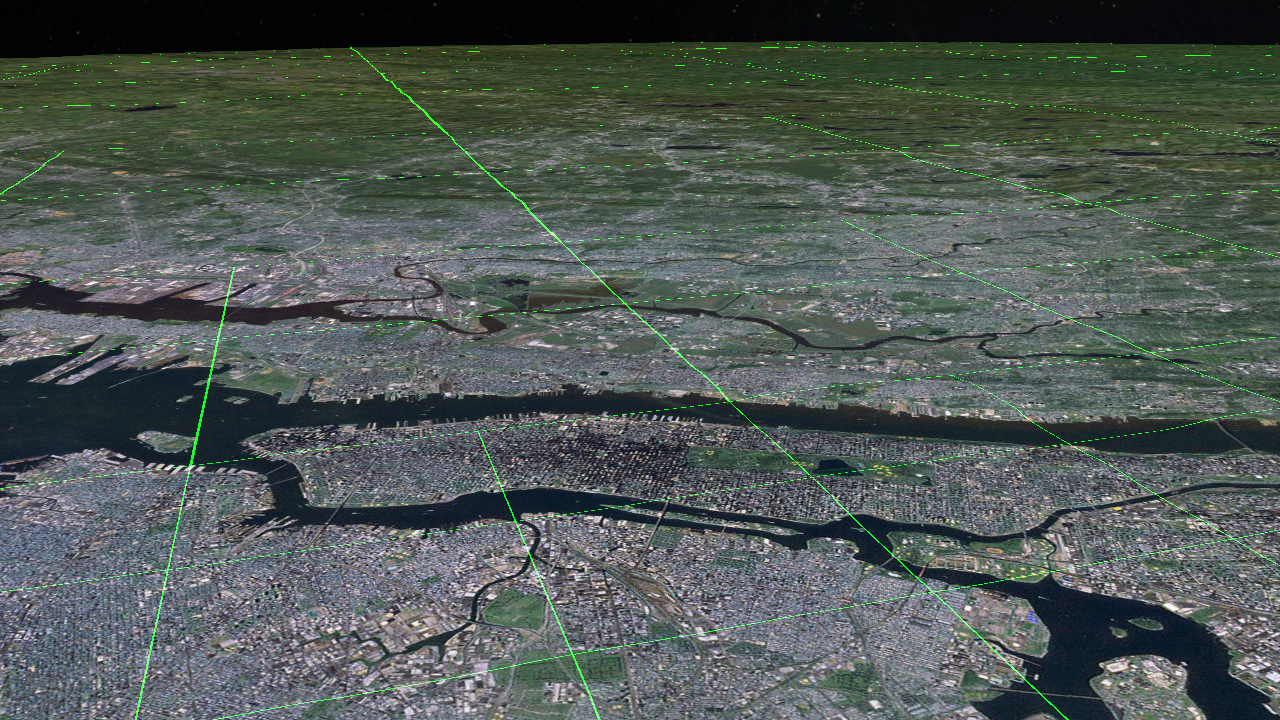
\includegraphics[width=\textwidth]{figures/results/culling/cam_d.png}
    \end{subfigure}
    \caption{Camera view looking over Brooklyn, Manhattan and New Jersey with distance based LOD}
    \label{fig:cullingdcam}
\end{figure}

\clearpage
\begin{figure}[h]
    \centering
    \begin{subfigure}[bt]{0.48\textwidth}
        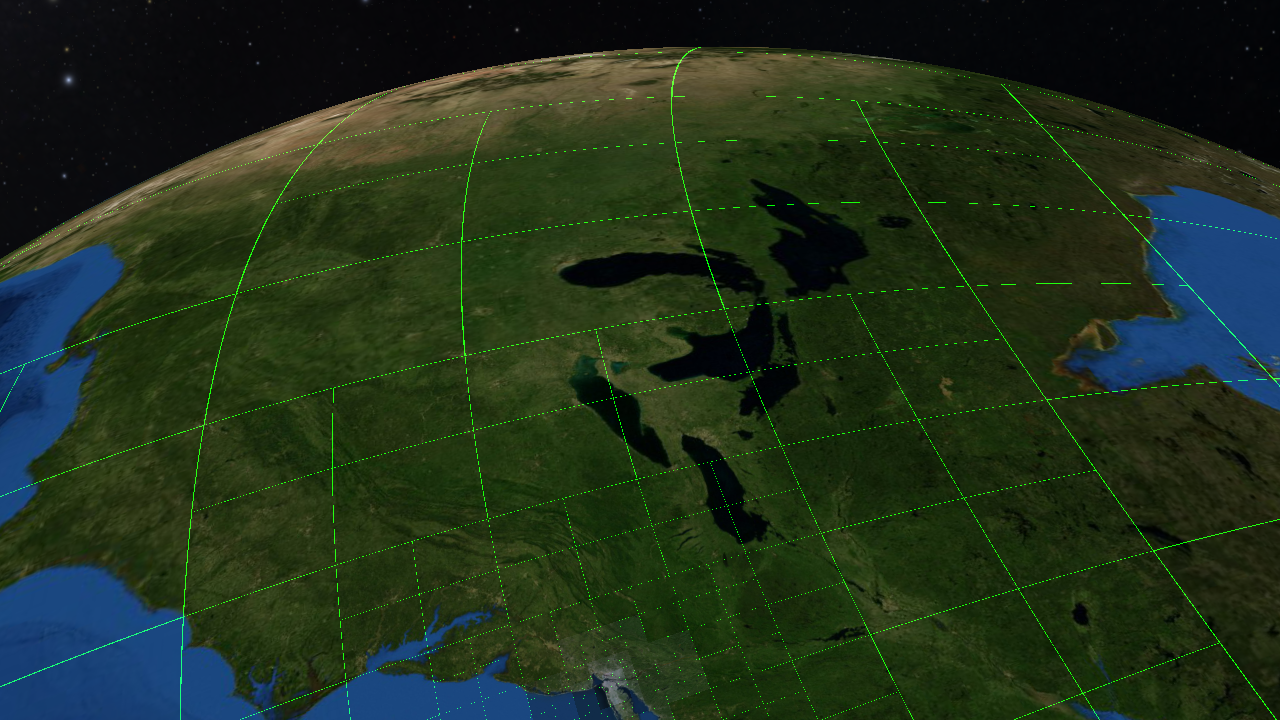
\includegraphics[width=\textwidth]{figures/results/culling/d.png}
        \caption{No culling}
    \end{subfigure}
    ~
    \begin{subfigure}[bt]{0.48\textwidth}
        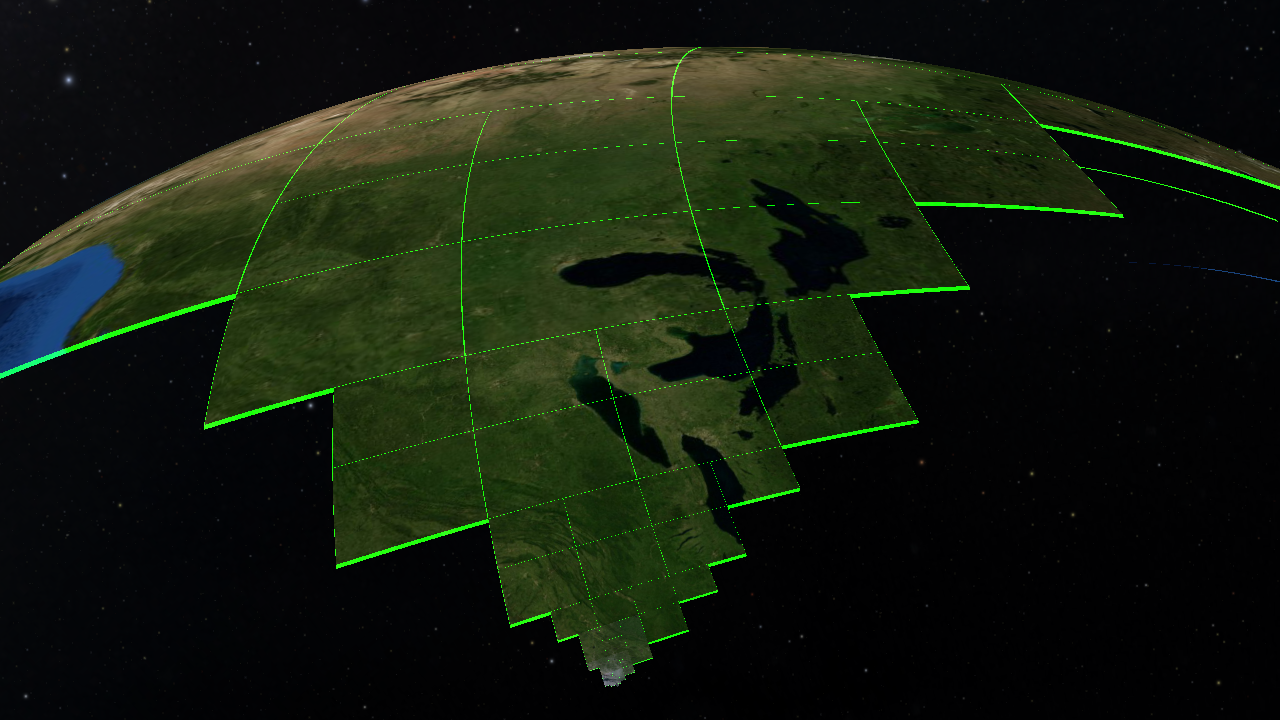
\includegraphics[width=\textwidth]{figures/results/culling/df.png}
        \caption{Frustum culling}
    \end{subfigure}
    ~
    \begin{subfigure}[bt]{0.48\textwidth}
        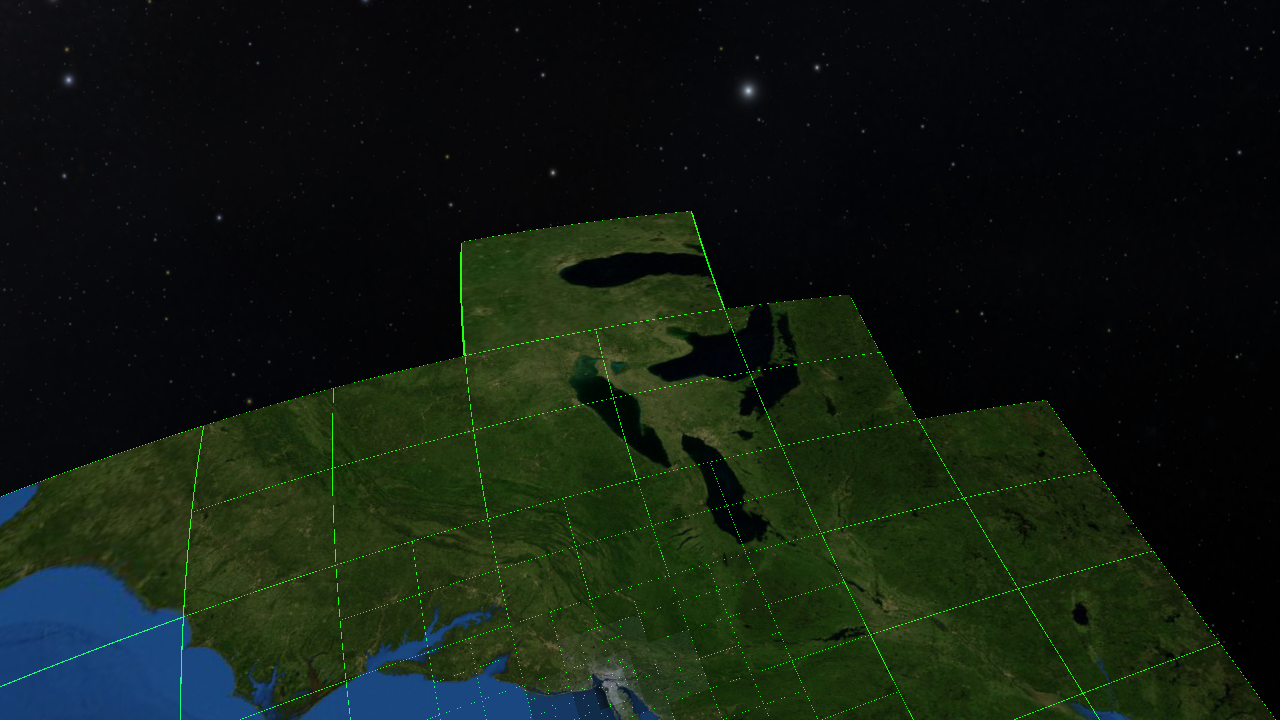
\includegraphics[width=\textwidth]{figures/results/culling/dh.png}
        \caption{Horizon culling}
    \end{subfigure}
    ~
    \begin{subfigure}[bt]{0.48\textwidth}
        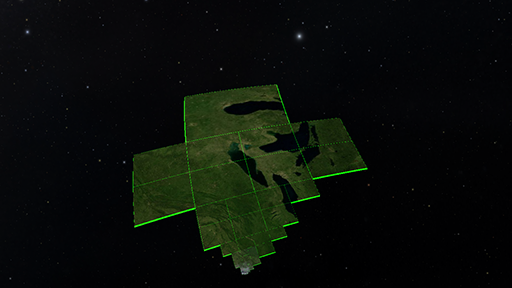
\includegraphics[width=\textwidth]{figures/results/culling/dhf.png}
        \caption{Frustum and Horizon culling}
    \end{subfigure}
    \caption{Demonstration of culling algorithms}
    \label{fig:cullingd}
\end{figure}

\begin{table}[h]
\centering
\caption[]{Culling for projected area based LOD}
  \label{table:cullingd}
  \begin{tabular}{| r | c c c c |}
    \hline
      \textbf{Culling}            & \textbf{None}  & \textbf{Horizon} & \textbf{Frustum}  & \textbf{Both} \\ \hline
      \textbf{Chunk nodes}        & 514            & 390              & 214               & 154 \\ 
      \textbf{Leaf chunk nodes}   & 386            & 293              & 161               & 116 \\ 
      \textbf{Rendered chunks}    & 386            & 254              & 79                & 53 \\
      \textbf{Frame Time}         & 155 ms         & 53 ms            & 39 ms             & 28 ms \\
      \textbf{Globe render time}  & 119 ms         & 30 ms            & 14 ms             & 10 ms \\
    \hline
  \end{tabular}
\end{table}

\clearpage
\section{Culling for Projected Area based LOD}
\FloatBarrier
The culling algorithms Frustum culling and Horizon Culling were compared and evaluated. The settings used are provided in Table \ref{table:cullinga}. Note that LOD evaluation is done by distance. Figure \ref{fig:cullingacam} shows the camera view evaluated. Figure \ref{fig:cullinga} shows and overview of the rendered chunks using the different culling and benchmarks are listed in Table \ref{table:cullinga}.

\begin{table}[h]
  \centering
  \caption[]{Culling test}
    \label{table:cullingd}
  \begin{tabular}{| r l |}
    \hline
      \textbf{Globe:}             & Earth \\
      \textbf{Map datasets:}      & HeightLayers=[GCS\_Elevation\footnote{http://services.arcgisonline.com/ArcGIS/rest/services/ESRI\_Imagery\_World\_2D/MapServer}] \\
                                  & ColorLayers=[ESRI\_World\_2D\footnote{http://198.102.45.23/arcgis/rest/services/worldelevation3d/terrain3d?}] \\
      \textbf{LOD Scale factor:}  & 7.8 \\
      \textbf{LOD Evaluation:}    & By Projected Area \\
      \textbf{Culling:}           & \textbf{Evaluated} \\
      \textbf{Level blending:}    & Enabled \\
      \textbf{Camera View:}       & Looking towards western horizon\\
      \textbf{Location:}          & New York, New Jersey\\
    \hline
  \end{tabular}
\end{table}

\begin{figure}[h]
    \centering
    \begin{subfigure}[bt]{1.0\textwidth}
        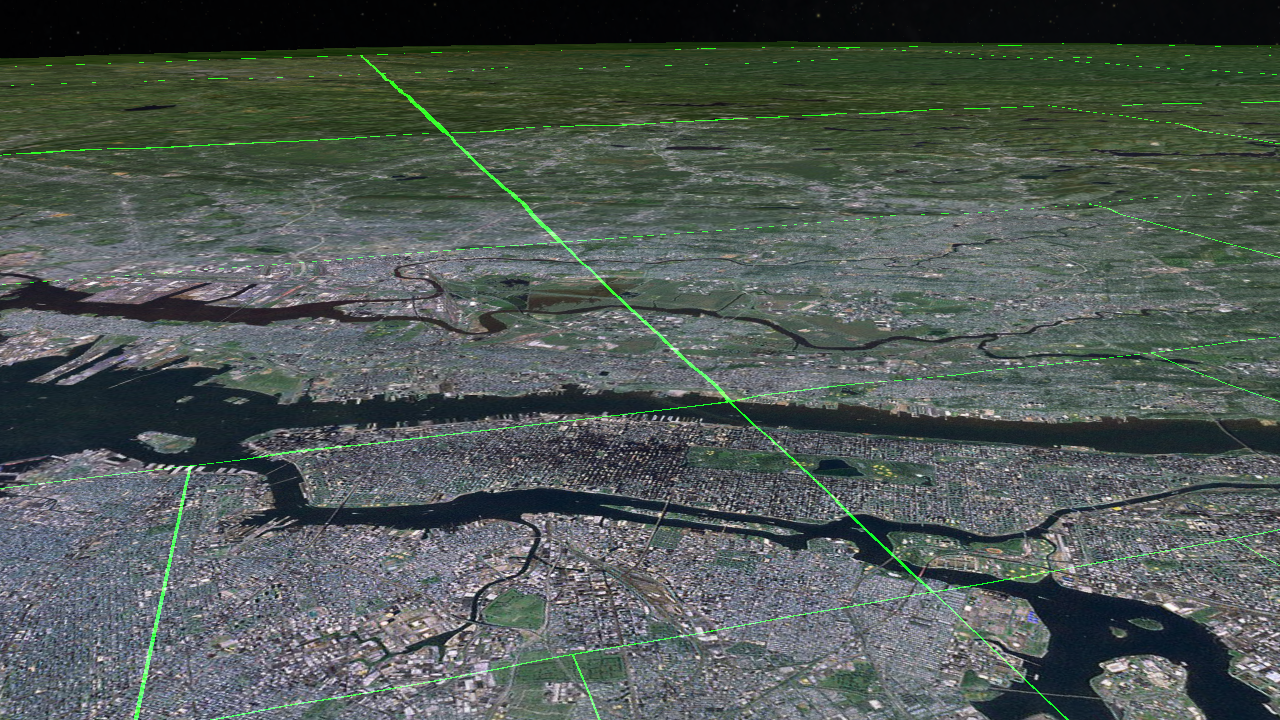
\includegraphics[width=\textwidth]{figures/results/culling/cam_a.png}
    \end{subfigure}
    \caption{Camera view looking over Brooklyn, Manhattan and New Jersey with Area based LOD}
    \label{fig:cullingacam}
\end{figure}

\clearpage
\begin{figure}[h]
    \centering
    \begin{subfigure}[bt]{0.48\textwidth}
        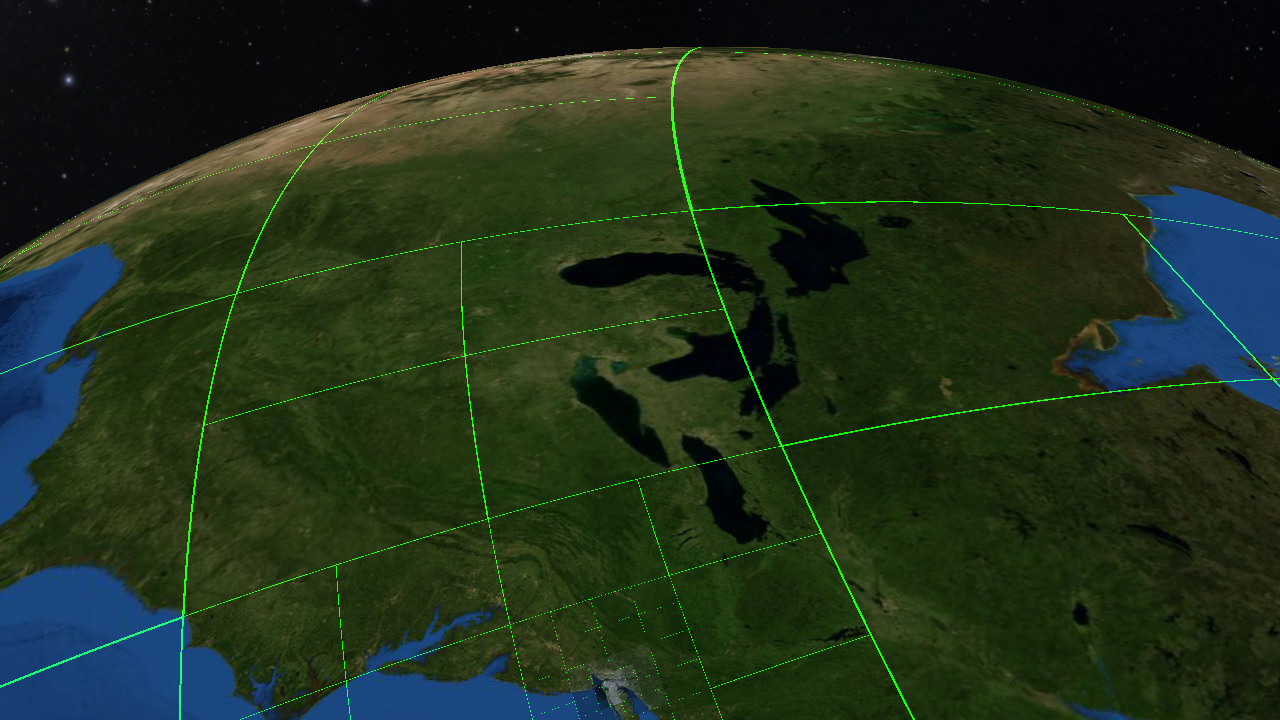
\includegraphics[width=\textwidth]{figures/results/culling/a.png}
        \caption{No culling}
    \end{subfigure}
    ~
    \begin{subfigure}[bt]{0.48\textwidth}
        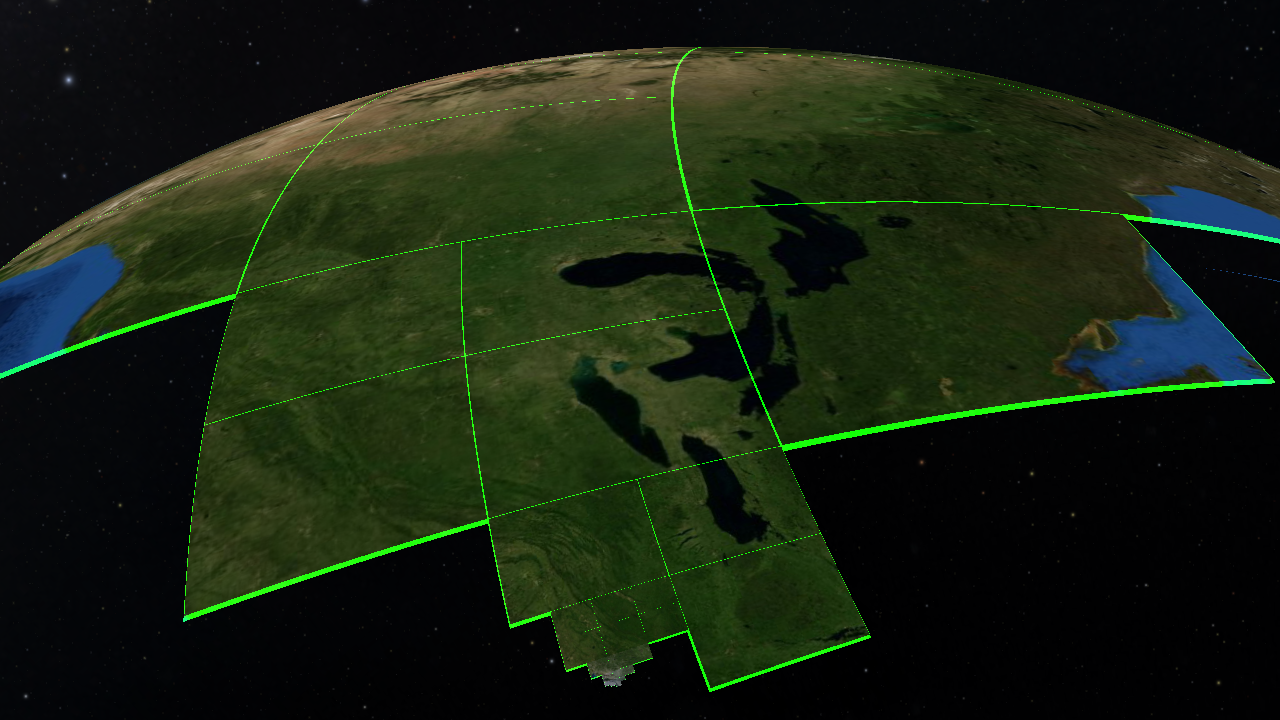
\includegraphics[width=\textwidth]{figures/results/culling/af.png}
        \caption{Frustum culling}
    \end{subfigure}
    ~
    \begin{subfigure}[bt]{0.48\textwidth}
        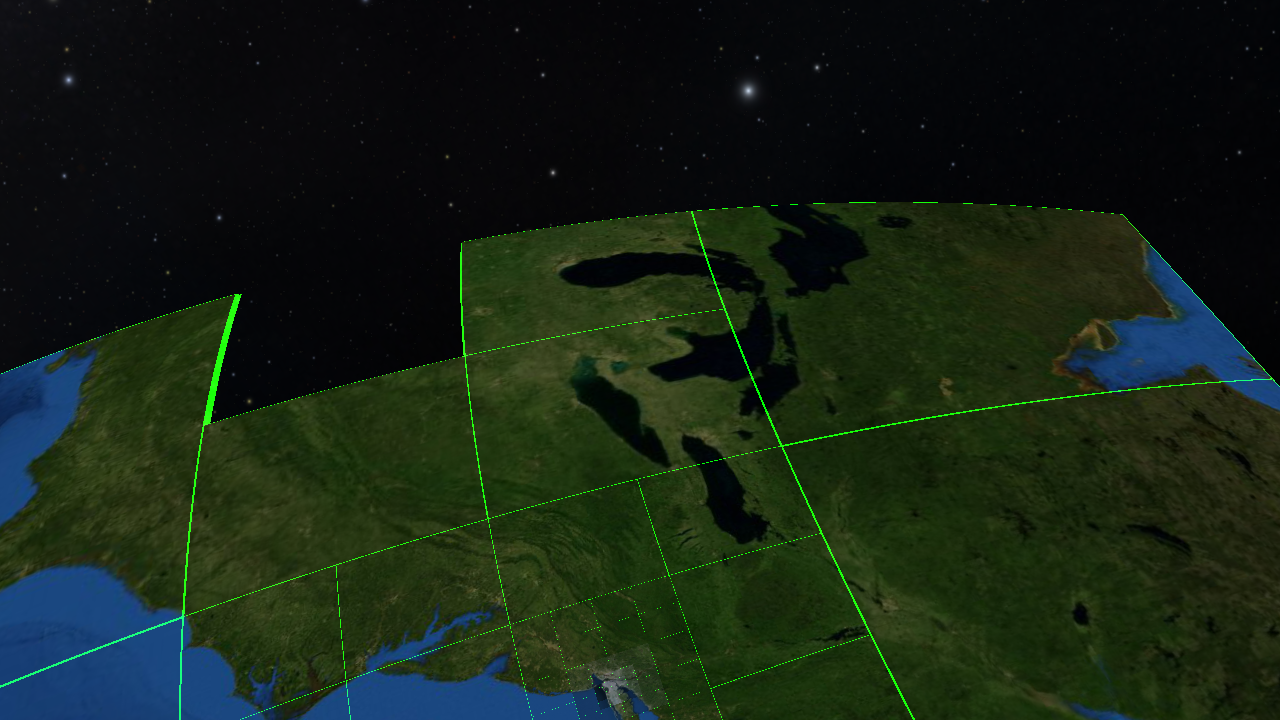
\includegraphics[width=\textwidth]{figures/results/culling/ah.png}
        \caption{Horizon culling}
    \end{subfigure}
    ~
    \begin{subfigure}[bt]{0.48\textwidth}
        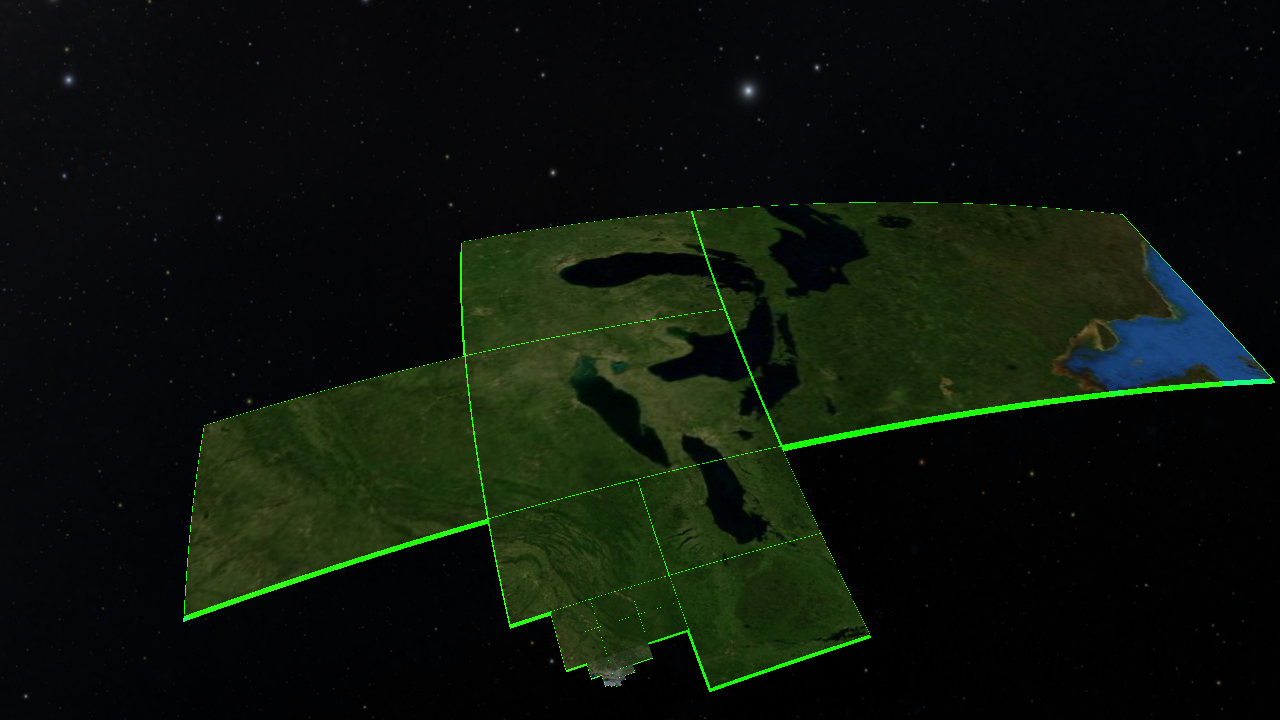
\includegraphics[width=\textwidth]{figures/results/culling/afh.png}
        \caption{Frustum and Horizon culling}
    \end{subfigure}
    \caption{Demonstration of culling algorithms}
    \label{fig:cullinga}
\end{figure}

\begin{table}[h]
\centering
\caption[]{Projcted area based}
  \label{table:cullinga}
  \begin{tabular}{| r | c c c c |}
    \hline
      \textbf{Culling}            & \textbf{None} & \textbf{Horizon}  & \textbf{Frustum}  & \textbf{Both} \\ \hline
      \textbf{Chunk nodes}        & 270           & 202               & 134               & 94 \\ 
      \textbf{Leaf chunk nodes}   & 203           & 152               & 101               & 71 \\ 
      \textbf{Rendered chunks}    & 203           & 133               & 43                & 26 \\
      \textbf{Frame Time}         & 123 ms        & 41 ms             & 30 ms             & 23 ms \\
      \textbf{Globe render time}  & 62 ms         & 16 ms             & 7.9 ms            & 5.6 ms \\
    \hline
  \end{tabular}
\end{table}

\clearpage
\section{Switching using level blending}
\FloatBarrier
The visual result of using the distance based level blending is shown in Figure \ref{fig:blending2}.
\begin{figure}[h]
    \centering
    \begin{subfigure}[bt]{0.48\textwidth}
        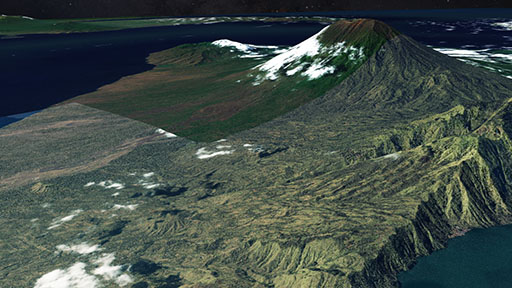
\includegraphics[width=\textwidth]{figures/results/blending/blending_bali2_disabled.jpg}
        \caption{No blending}
    \end{subfigure}
    \begin{subfigure}[bt]{0.48\textwidth}
        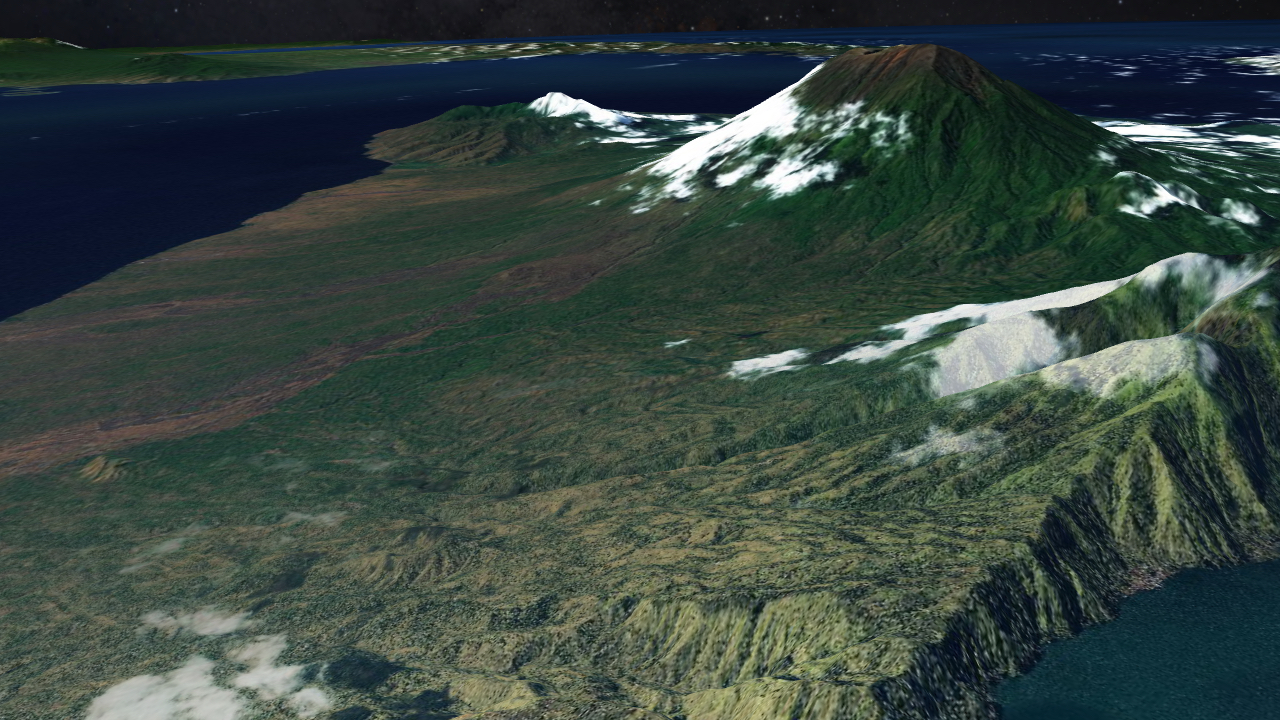
\includegraphics[width=\textwidth]{figures/results/blending/blending_bali2_enabled.jpg}
        \caption{Distance based level blending}
    \end{subfigure}
    \caption{Comparison of level blending and no blending. The LOD scale factor is set low to show the resolution penalty of using blending.}
    \label{fig:blending2}
\end{figure}


A performance benchmark of the blending algorithm is described below. Note that the in order to see the pixel resolution penalty of using level blending with the bear eye, the LOD scale factor was tuned down enough 

\begin{table}
  \centering
  \caption[]{Benchmark: Level blending}
    \label{table:levelblending}
  \begin{tabular}{| r l |}
    \hline
      \textbf{Globe:}             & Earth \\
      \textbf{Map datasets:}      & HeightLayers=[GCS\_Elevation\footnote{http://services.arcgisonline.com/ArcGIS/rest/services/ESRI\_Imagery\_World\_2D/MapServer}] \\
                                  & ColorLayers=[ESRI\_World\_2D\footnote{http://198.102.45.23/arcgis/rest/services/worldelevation3d/terrain3d?}] \\
      \textbf{LOD Scale factor:}  & 4.65 \\
      \textbf{LOD Evaluation:}    & By distance \\
      \textbf{Culling:}           & Frustum culling, Horizon culling \\
      \textbf{Camera View:}       & Horizon \\
    \hline
  \end{tabular}
\end{table}

\begin{figure}[h]
    \centering
    \begin{subfigure}[bt]{0.48\textwidth}
        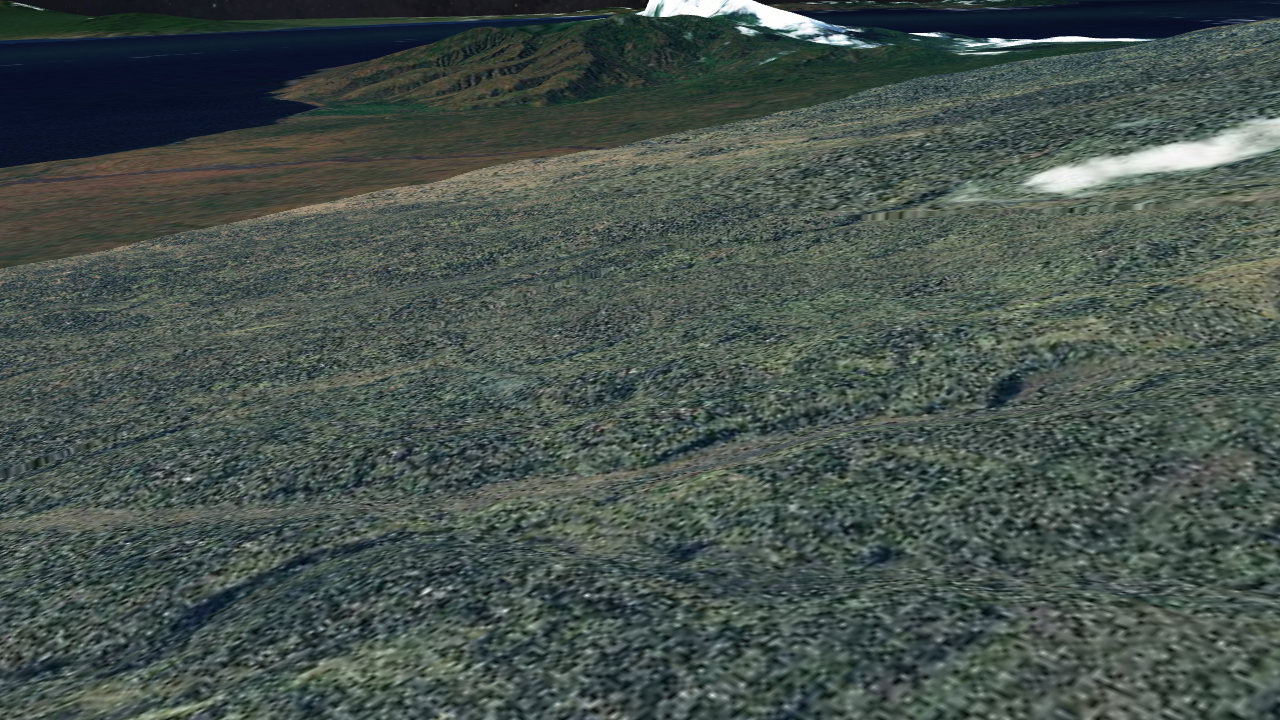
\includegraphics[width=\textwidth]{figures/results/blending/blending_bali_disabled.jpg}
        \caption{No blending}
    \end{subfigure}
    \begin{subfigure}[bt]{0.48\textwidth}
        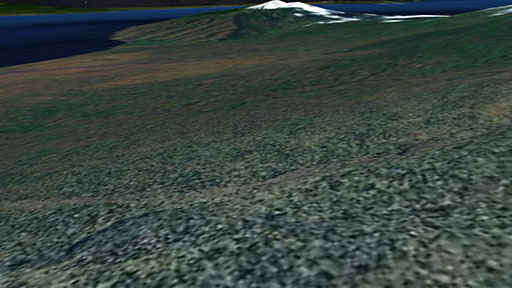
\includegraphics[width=\textwidth]{figures/results/blending/blending_bali_enabled.jpg}
        \caption{Level blending}
    \end{subfigure}
    \caption{Comparison of level blending and no blending. The LOD scale factor is set low to show the resolution penalty of using blending.}
    \label{fig:blending}
\end{figure}

\begin{table}
\centering
\caption[]{Top down settings}
  \label{table:resultblending}
  \begin{tabular}{| r | c c |}
    \hline
      \textbf{Figure \ref{fig:blending}}  & \textbf{No blending} & \textbf{Level blending} \\ \hline
      \textbf{Samples per fragment} & 1 & 3 \\ 
      \textbf{Avg. globe render time}  & 10.3 ms & 10.1 ms \\ 
      \textbf{Avg. frame time}  & 40 ms &  49 ms \\ 
      \textbf{Screenshot jpg size} & 1,1 MB & 0,7 MB \\
    \hline
  \end{tabular}
\end{table}

\clearpage
\section{Polar Pinching}
\FloatBarrier
The impact of polar pinching on the chunk tree was evaluated using both Distance based LOD and Area based LOD. The results are presented in Figure \ref{fig:pincheval}.


\begin{table}[h]
  \centering
  \caption[]{Evaluating pinching}
    \label{table:pinchingstart}
  \begin{tabular}{| r l |}
    \hline
      \textbf{Globe:}             & Earth \\
      \textbf{Map datasets:}      & HeightLayers=[GCS\_Elevation\footnote{http://services.arcgisonline.com/ArcGIS/rest/services/ESRI\_Imagery\_World\_2D/MapServer}] \\
                                  & ColorLayers=[ESRI\_World\_2D\footnote{http://198.102.45.23/arcgis/rest/services/worldelevation3d/terrain3d?}] \\
      \textbf{LOD Scale factor:}  & 10.0 \\
      \textbf{LOD Evaluation:}    & Evaluated \\
      \textbf{Culling:}           & Frustum culling, Horizon culling \\
      \textbf{Camera View:}       & Facing down\\
      \textbf{Location:}          & Quito, Ecuador and North Pole\\
    \hline
  \end{tabular}
\end{table}

\iffalse
\begin{table}[h]
\centering
\caption[]{Evaluation of polar pinching with Distance based LOD}
  \label{table:polarpinching}
  \begin{tabular}{| r | c c |}
    \hline
      \textbf{Distance based LOD} & \textbf{Equator} & \textbf{North Pole} \\ \hline
      \textbf{Chunk nodes}        & 78           & 506               \\ 
      \textbf{Leaf chunk nodes}   & 59           & 380                \\ 
      \textbf{Rendered chunks}    & 6            & 151                \\
      \textbf{Frame Time}         & ? ms         & ? ms              \\
      \textbf{Globe render time}  & 2,7 ms       & 31 ms              \\
    \hline
  \end{tabular}
\end{table}
\fi


\begin{figure}[h]
\begin{tikzpicture}
    \begin{axis}[
        width  = 1.0*\textwidth,
        height = 8cm,
        major x tick style = transparent,
        ybar=2*\pgflinewidth,
        bar width=14pt,
        ymajorgrids = true,
        %ylabel = {Number of},
        symbolic x coords={D: Equator, D: Pole, A: Equator, A: Pole},
        xtick = data,
        scaled y ticks = false,
        enlarge x limits=0.25,
        ymin=0,
        legend cell align=left,
        legend style={
                at={(0.98, 0.60)},
                anchor=south east,
                column sep=1ex
        }
    ]

      \addplot[style={chunks_color,fill=chunks_color,mark=none}]
        coordinates { (D: Equator, 78) (D: Pole, 506) (A: Equator, 94) (A: Pole, 250) };

      \addplot[style={leafs_color,fill=leafs_color,mark=none}]
        coordinates { (D: Equator, 59) (D: Pole, 380) (A: Equator, 94) (A: Pole, 188) };
      
      \addplot[style={rendered_color,fill=rendered_color,mark=none}]
        coordinates { (D: Equator, 6) (D: Pole, 151) (A: Equator, 17) (A: Pole, 64) };

      \addplot[style={globe_render_time,fill=globe_render_time,mark=none}]
        coordinates { (D: Equator, 27) (D: Pole, 310) (A: Equator, 43) (A: Pole, 140) };

      \legend{Chunks, Leaf chunks, Rendered chunks, Render time [$10^{-4}$ s]}

    \end{axis}
\end{tikzpicture}
\caption{Comparison of Distance based and Area based LOD at the Equator and the North Pole. \textbf{D} = Distance based LOD, \textbf{A} = Area based LOD.}
\label{fig:pincheval}
\end{figure}

\iffalse
\begin{table}[h]
\centering
\caption[]{Evaluation of polar pinching with Area based LOD}
  \label{table:polarpinching}
  \begin{tabular}{| r | c c |}
    \hline
      \textbf{Area based LOD}     & \textbf{Equator} & \textbf{North Pole} \\ \hline
      \textbf{Chunk nodes}        & 94           & 250               \\ 
      \textbf{Leaf chunk nodes}   & 71           & 188                \\ 
      \textbf{Rendered chunks}    & 17           & 64                \\
      \textbf{Frame Time}         & ? ms         & ? ms              \\
      \textbf{Globe render time}  & 4,3 ms       & 14 ms              \\
    \hline
  \end{tabular}
\end{table}
\fi

\clearpage
\section{Benchmark: Interactive Globe Browsing}
\FloatBarrier
The purpose of the globe browsing is be able to interactively explore virtual globes and map datasets. In order to captures how the system behaves over time, a user interaction sequence was evaluated. The sequence is described step by step below, and illustrated in Figure \ref{fig:interaction}.

\begin{enumerate}
  \item Camera views Earth from space
  \item Descend down to Naturpark Karwendel, north of Innsbruck, Austria
  \item Tilt camera up, view north horizon
  \item Turn camera 180 degrees, view south horizon
  \item Tilt camera down
\end{enumerate}

\begin{figure}[h]
    \centering
    \begin{subfigure}[bt]{1.0\textwidth}
        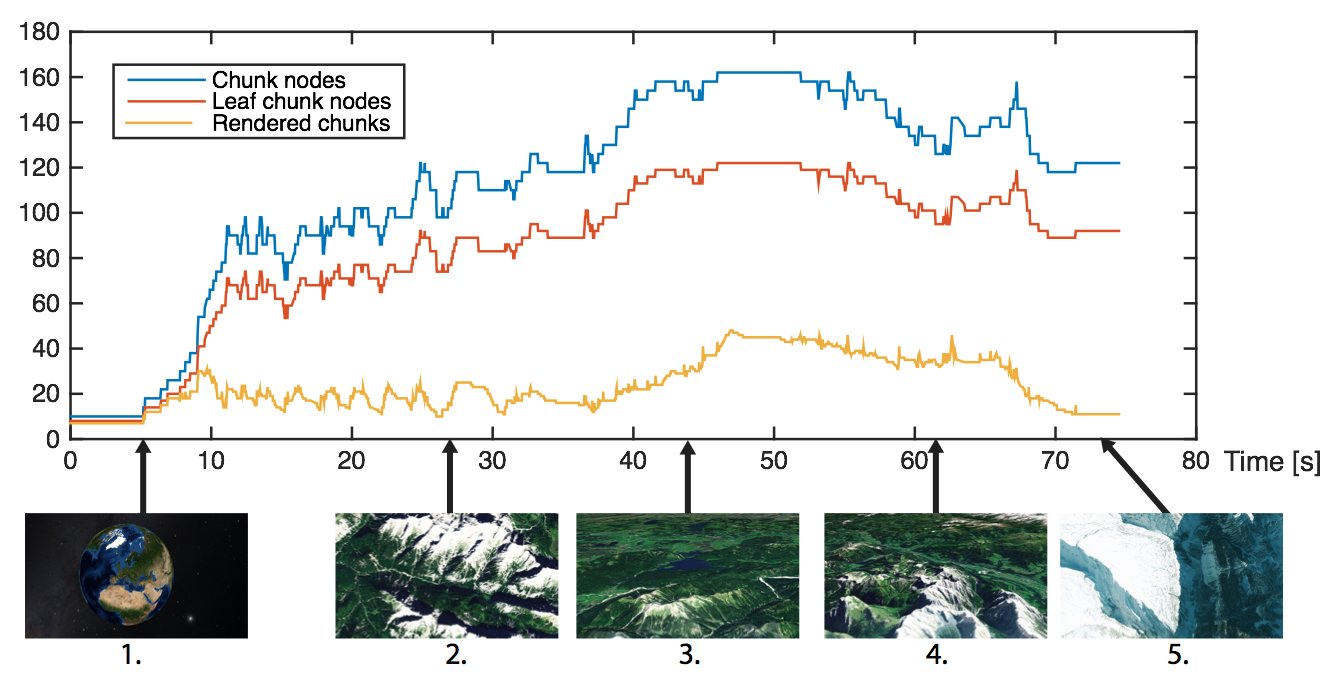
\includegraphics[width=\textwidth]{figures/results/globebrowsing.png}
    \end{subfigure}
    \caption{Chunk tree over time.}
    \label{fig:interaction}
\end{figure}

\section{Screenshots}
\FloatBarrier
